% Author: Seongjin Lee 
% Gyeongsang National University, Korea 
% 
% 2021-02-27
%

\documentclass[newPxFont,sthlmFooter,nooffset]{beamer}
\usepackage{kotex}
%\usetheme{sthlm}
\usepackage{../style/beamerthemesthlm}
\hypersetup{pdfauthor={Seongjin Lee (insight@gnu.ac.kr)},
            pdfsubject={Data Structure and Algorithm, Lecture Note},
            pdfkeywords={Data Structure, Algorithm, Lecture, Note},
            pdfmoddate={D: \pdfdate},
            pdfcreator={Seongjin Lee}}

%\setbeamertemplate{footline}[text line]{%
%    \parbox{\linewidth}{\vspace*{-8pt} \insertsectionhead  \hfill\insertshortauthor\hfill\insertpagenumber}}
%\setbeamertemplate{navigation symbols}{}

\usepackage{tkz-graph}
\usetikzlibrary{matrix, backgrounds}
\setbeamertemplate{blocks}[rounded]
\usepackage{mathtools}

\title{Data Structure and Algorithm}
\subtitle{Class 11}
\author[SJL]{Seongjin Lee}
\institute{\href{mailto:insight@gnu.ac.kr}{insight@gnu.ac.kr}\\\url{http://resourceful.github.io}\\Systems Research Lab.\\GNU}
\date{2021-02-27} 

\begin{document}

\lstset{basicstyle=\normalsize\ttfamily, language=C}

\frame[plain,t]{\titlepage} 

\frame[t]{\frametitle{Table of contents}\tableofcontents} 


%---------------------------------------------------------

\section{Sorting}

\begin{frame}[t]
  \frametitle{Sorting}
Types of Sorting
\begin{itemize}
\item Internal Sorting - The list is small enough to sort entirely in main memory
\item External Sorting - The list is too large to sort in main memory
\end{itemize}

Internal sorting algorithms

\begin{itemize}
\item Bubble sort
\item Selection sort
\item Insertion sort
\item Quick sort
\item Shell sort
\item Heap sort
\item Radix sort
\end{itemize}
\end{frame}

\section{Bubble sort}


\begin{frame}[t, fragile]
  \frametitle{Bubble sort}
  \begin{lstlisting}
repeat until no swaps
    for i from 0 to n-2
        if ith and i+1th elements out of order
            swap them
  \end{lstlisting}
\end{frame}
% add horizontal line -KSS-
\begin{frame}[t]
  \frametitle{Bubble sort: example}
  \begin{tabular}{p{1.5cm}|| c | c | c | c | c | c | c |p{4cm}}
%11, 12 line revised -7p KSS-
initial & 15 & 4  & 8  & 3  & 50 & 9 & 20 & unsorted array \\ \hline
$1^{st}$ run & \color{red} 4  & \color{red}15 & 8  & 3  & 50 & 9 & 20 & cmp 1 and 2, swap \pause\\  \hline
$1^{st}$ run & 4  & \color{red}8  & \color{red}15 & 3  & 50 & 9 & 20 & cmp 2 and 3, swap \pause \\ \hline
$1^{st}$ run & 4  & 8  & \color{red}3  & \color{red}15 & 50 & 9 & 20 & cmp 3 and 4, swap \pause \\ \hline
$1^{st}$ run & 4  & 8  & 3  & 15 & 50 & 9 & 20 & cmp 4 and 5, no swap \pause \\ \hline
$1^{st}$ run & 4  & 8  & 3  & 15 & \color{red}9 & \color{red}50 & 20 & cmp 5 and 6, swap \pause \\ \hline
$1^{st}$ run & 4  & 8  & 3  & 15 & 9 & \color{red}20 & \color{red}50 & cmp 6 and 7, swap \pause \\ \hline
$2^{nd}$ run & 4  & 8  & 3  & 15 & 9 & 20 & \color{blue}50 & cmp 1 and 2, no swap  \\ \hline
$2^{nd}$ run & 4  & \color{red}3  & \color{red}8  & 15 & 9 & 20 & \color{blue}50 & cmp 2 and 3,  swap  \\ \hline
$2^{nd}$ run & 4  & 3  & 8  & 15 & 9 & 20 & \color{blue}50 & cmp 3 and 4, no swap  \\ \hline
$2^{nd}$ run & 4  & 3  & 8  & \color{red}9  & \color{red}15 & 20 & \color{blue}50 & cmp 4 and 5, swap  \\ \hline
$2^{nd}$ run & 4  & 3  & 8  & 9  & 15 & \color{blue}20 & \color{blue}50 & cmp 5 and 6, no swap  \\ \hline
$3^{rd}$ run & \color{red}3  & \color{red}4  & 8  & 9  & \color{blue}15 & \color{blue}20 & \color{blue}50 & 1, 2 swap  \\ \hline
$4^{th}$ run & 3  & 4  & 8  & \color{blue}9  & \color{blue}15 & \color{blue}20 & \color{blue}50 & no swap  \\ \hline
$5^{th}$ run & 3  & 4  & \color{blue}8  & \color{blue}9  & \color{blue}15 & \color{blue}20 & \color{blue}50 & no swap  \\ \hline
$6^{th}$ run & 3  & \color{blue}4  & \color{blue}8  & \color{blue}9  & \color{blue}15 & \color{blue}20 & \color{blue}50 & no swap  \\ 
  \end{tabular}
\end{frame}



\begin{frame}[t, fragile, allowframebreaks]
  \frametitle{Bubble sort: the code (\texttt{codes/bubble.c})}
   \lstset{basicstyle=\normalsize, keywordstyle=\color{blue}, language=C}
  \lstinputlisting{codes/bubble.c}

\end{frame}

\begin{frame}[t]
  \frametitle{Bubble sort: Time complexity}
%add horizontal line, adjust font size -12p KSS-
\begin{center}
  \begin{tabular}{c | p{3cm}}
    loop & \scriptsize{number of comparison} \\ \hline
    1    & n-1 \\
    2    & n-2 \\
    3    & n-3 \\
 $\cdot$ &  $\cdot$ \\
 $\cdot$ &  $\cdot$ \\
 $\cdot$ &  $\cdot$ \\
    n-1  &  1 \\
  \end{tabular}
\end{center}
%add youtube link -12p KSS-
Time complexity: $O(n^2)$
  
   \vspace{10mm}
\url{https://www.youtube.com/watch?v=lyZQPjUT5B4&t=50}
\end{frame}


\section{Selection sort}

\begin{frame}[t, fragile]
  \frametitle{Selection sort}

  \begin{lstlisting}
for i from 0 to n-1
    find smallest element between ith and n-1th
    swap smallest with ith element
  \end{lstlisting}  
\end{frame}


\begin{frame}[t, fragile]
  \frametitle{Selection sort}
  % add horizontal line -KSS-
  \begin{tabular}{p{1.5cm}|| c | c | c | c | c | c | c |p{4cm}}
initial & 15 & 4  & 8  & 3  & 50 & 9 & 20 & unsorted array \\ \hline
$1^{st}$ run & \color{red}3  & 4 & 8  & \color{red}15  & 50 & 9 & 20 & midx 15, min 3, swap \pause\\ [0.8em] \hline
$2^{nd}$ run & \color{blue}3  & \color{red}4 & 8  & 15  & 50 & 9 & 20 & midx 4, min 4 \pause\\  [0.8em] \hline
$3^{rd}$ run & \color{blue}3  & \color{blue}4 & \color{red}8  & 15  & 50 & 9 & 20 & midx 8, min 8 \pause\\  [0.8em] \hline
$4^{th}$ run & \color{blue}3  & \color{blue}4 &\color{blue} 8  & \color{red}9  & 50 & \color{red}15 & 20 & midx 15, min 9, swap \pause\\  [0.8em] \hline
$4^{th}$ run & \color{blue}3  & \color{blue}4 &\color{blue} 8  & \color{blue}9  & \color{red}15 & \color{red}50 & 20 & midx 50, min 15, swap \pause\\  [0.8em] \hline
$5^{th}$ run & \color{blue}3  & \color{blue}4 &\color{blue} 8  & \color{blue}9  & \color{blue}15 & \color{red}20 & \color{red}50 & midx 50, min 20, swap \\  [0.8em]
  \end{tabular}

\end{frame}


\begin{frame}[t, fragile]
  \frametitle{Selection sort: the Code (\texttt{codes/selection.c})}
  \lstinputlisting[firstnumber=38, firstline=38, lastline=51]{codes/selection.c}

\end{frame}
%add new page -17p KSS-
\begin{frame}[t]
	\frametitle{Select sort: Time complexity}
	\begin{center}
		\begin{tabular}{c | p{3cm}}
			loop & \scriptsize{number of comparison} \\ \hline
			1    & n-1 \\
			2    & n-2 \\
			3    & n-3 \\
			$\cdot$ &  $\cdot$ \\
			$\cdot$ &  $\cdot$ \\
			$\cdot$ &  $\cdot$ \\
			n-1  &  1 \\
		\end{tabular}
	\end{center}
	Time complexity: $O(n^2)$
\end{frame}

\section{Insertion sort}

\begin{frame}[t, fragile]
  \frametitle{Insertion sort}
  \begin{lstlisting}
for i from 1 to n-1
    call 0th through i-1th elements the ``sorted side''
    remove ith element
    insert it into sorted side in order
  \end{lstlisting}  
\end{frame}

\begin{frame}[t, fragile]
  \frametitle{Insertion sort}
  % restructure table -20p KSS-
  \begin{table}
  	\centering
  	
\begin{tabular}{c || c | c | c | c | c | p{4.5cm}}
  index   & 1  & 2  & 3  & 4  & 5  & ~ \\ \hline
  initial state& 36 & 28 & 30 & 17 & 23 & \\ \hline
  $1^{st}$ run& \color{red}28 & \color{red}36 & 30 & 17 & 23 & {\footnotesize 28 is smaller than 36, move 28 to the sorted side} \pause \\  \hline
  $2^{nd}$ run& \color{red}28 & \color{red}30 & \color{red}36 & 17 & 23 & {\footnotesize 30 is smaller than 36, move it to the sorted side} \pause \\  \hline
  $3^{rd}$ run& \color{red}17 & \color{red}28 & \color{red}30 & \color{red}36 & 23 & {\footnotesize 17 is smaller than 36, 30, and 28, move it to the sorted side} \pause \\  \hline
  $4^{th}$ run& \color{red}17 & \color{red}23 & \color{red}28 & \color{red}30 & \color{red}36 & {\footnotesize 23 is smaller than 36, 30, and 28, move it to the sorted side} 
\end{tabular}

\end{table}
\end{frame}


\begin{frame}[t, fragile]
  \frametitle{Insertion sort: the Code (\texttt{codes/insertion.c})}
  \lstinputlisting[firstnumber=29, firstline=29, lastline=41]{codes/insertion.c}

Time complexity: worst case $O(n^2)$, best case $O(n)$
\end{frame}


\section{Shell Sort}
\begin{frame}[t]
  \frametitle{Shell sort}
Shell sort is based on insertion sort algorithm to reduce the number of shifts. For example, if the list in decreasing order and we want to sort in increasing order, the far left record has to be moved to the far left, one by one.

\url{https://www.youtube.com/watch?v=1yDcmjLTWOg}
\end{frame}

\begin{frame}[t, fragile]
  \frametitle{Shell sort: the Code (\texttt{codes/shell.c})}
  \lstinputlisting[firstnumber=34, firstline=34, lastline=41]{codes/shell.c}


\end{frame}

\begin{frame}[t, fragile]
  \frametitle{Shell sort: the Code (\texttt{codes/shell.c})}
  \lstinputlisting[firstnumber=43, firstline=43, lastline=51]{codes/shell.c}
  %add time conplexity -25p KSS-
time complexity: worst case $O(n^2)$, best case $O(n)$

\end{frame}


\section{Quick Sort}



\begin{frame}[t, fragile]
  \frametitle{Quick Sort}
Divide and Conquer
\begin{itemize}
\item two phase
\item split and control
\end{itemize}

Using recursion
\begin{itemize}
\item stack is needed
\end{itemize}

Best average time
\begin{itemize}
\item $O(n\cdot log_2n)$
\end{itemize}
\end{frame}


\begin{frame}[t, fragile]
  \frametitle{Quick sort: The principle}
  \begin{enumerate}
  \item Pick a ``\textbf{pivot}'' element
  \item ``\textbf{partition}'' the array into \textit{three} parts
    \begin{itemize}
    \item $1^{st}$ part: all elements in this is less than the pivot
    \item $2^{nd}$ part: the pivot itself (only one element)
    \item $3^{rd}$ part: all elements in this part is greater than or equal to the pivot
    \end{itemize}
  \item Recursively apply quick sort to the first and the third part
    \begin{itemize}
    \item swap the out of order entries from the first and the third part
    \end{itemize}
  \end{enumerate}


\end{frame}

\newcounter{listcount} \newcounter{totcount}
%\setlength{\fboxsep}{0.5pt}%

\newcommand{\printarray}[2][1em]{% \printarray[<width>]{<array list>}
  \unskip \setcounter{totcount}{0}% Reset totcount counter
  \renewcommand*{\do}[1]{\stepcounter{totcount}}% Count elements
  \docsvlist{#2}% Process list a first time to obtain # of elements
  \setcounter{listcount}{0}% Reset listcount counter
  \renewcommand*{\do}[1]{%
    \stepcounter{listcount}% Move to next element
    \framebox[#1][c]{\rule{0pt}{1.5ex}\smash{\ensuremath{##1}}}%
    \ifnum\value{listcount}<\value{totcount}\thickspace\fi
  }
  \docsvlist{#2}% Process list a second time to typeset each element
}

\begin{frame}[t, fragile]
  \frametitle{Quick Sort}
Initial list \printarray[2em]{31, 11, 41, 12, 51, 90, 20, 64, 53, 55, 32}

\[
\underbracket[0.5pt]{{\thickspace}\printarray[2em]{\color{red}31, 11, \color{blue}41, 12, 51, 90, \color{blue}20, 64, 53, 55, \color{red}32}{\thickspace}}_{pivot=31}
\]
\begin{itemize}
\item examine the first, and last item of the full list that is 31 (first, pivot), and 32 (last)
\item Search forward until we find an item larger than the pivot $41 > 31$
\item Search backward until we find an item smaller than the pivot $20 < 31$
\item Swap the two items
\end{itemize}

\[
\underbracket[0.5pt]{{\thickspace}\printarray[2em]{\color{red}31, 11, \color{blue}20, 12, 51, 90, \color{blue}41, 64, 53, 55, \color{red}32}{\thickspace}}_{pivot=31}
\]
\end{frame}


\begin{frame}[t, fragile]
  \frametitle{Quick Sort}
\[
\underbracket[0.5pt]{{\thickspace}\printarray[2em]{\color{red}31, 11, \color{blue}20, 12, 51, 90, \color{blue}41, 64, 53, 55, 32}{\thickspace}}_{pivot=31}
\]
\begin{itemize}
\item Repeat the process until the left and right indices cross each other
\item Then swap the item with the pivot
\end{itemize}
\[
\underbracket[0.5pt]{{\thickspace}\printarray[2em]{12, 11, \color{blue}20, \color{red}31, 51, 90, \color{blue}41, 64, 53, 55, 32}{\thickspace}}_{pivot=31}
\] 
\end{frame}


\begin{frame}[t, fragile]
  \frametitle{Quick Sort}
\[
\underbracket[0.5pt]{{\thickspace}\printarray[2em]{12, 11, 20}{\thickspace}}_{left}
\underbracket[0.5pt]{{\thickspace}\printarray[2em]{\color{red}31}{\thickspace}}_{pivot}
\underbracket[0.5pt]{{\thickspace}\printarray[2em]{51, 90, 41, 64, 53, 55, 32}{\thickspace}}_{right}
\] 

\begin{itemize}
\item Repeat the quick sort for the left and right part
\end{itemize}

\[
\underbracket[0.5pt]{{\thickspace}\printarray[2em]{12, 11, 20}{\thickspace}}_{left}
\underbracket[0.5pt]{{\thickspace}\printarray[2em]{\color{red}31}{\thickspace}}_{pivot}
\color{black!50}\underbracket[0.5pt]{{\thickspace}\printarray[2em]{51, 90, 41, 64, 53, 55, 32}{\thickspace}}_{right}
\] \pause
\[
\underbracket[0.5pt]{
\underbracket[0.5pt]{{\thickspace}\printarray[2em]{12}{\thickspace}}_{left} 
\underbracket[0.5pt]{{\thickspace}\printarray[2em]{\color{red}11}{\thickspace}}_{pivot}
\underbracket[0.5pt]{{\thickspace}\printarray[2em]{ 20}{\thickspace}}_{right}
}_{left}
\underbracket[0.5pt]{{\thickspace}\printarray[2em]{\color{red}31}{\thickspace}}_{pivot}
\color{black!50}\underbracket[0.5pt]{{\thickspace}\printarray[2em]{51, 90, 41, 64, 53, 55, 32}{\thickspace}}_{right}
\] \pause
\[
\underbracket[0.5pt]{
\underbracket[0.5pt]{{\thickspace}\printarray[2em]{\color{red}11}{\thickspace}}_{left} 
\underbracket[0.5pt]{{\thickspace}\printarray[2em]{\color{red}12}{\thickspace}}_{pivot}
\underbracket[0.5pt]{{\thickspace}\printarray[2em]{\color{red}20}{\thickspace}}_{right}
}_{left}
\underbracket[0.5pt]{{\thickspace}\printarray[2em]{\color{red}31}{\thickspace}}_{pivot}
\color{black!50}\underbracket[0.5pt]{{\thickspace}\printarray[2em]{51, 90, 41, 64, 53, 55, 32}{\thickspace}}_{right}
\] 



\end{frame}

\begin{frame}[t, fragile]
  \frametitle{Quick Sort}
\[
{\color{black!50}\underbracket[0.5pt]{{\thickspace}\printarray[2em]{11, 12, 20}{\thickspace}}_{left}}
\underbracket[0.5pt]{{\thickspace}\printarray[2em]{\color{red}31}{\thickspace}}_{pivot}
\underbracket[0.5pt]{{\thickspace}\printarray[2em]{\color{red}51, 90, 41, 64, 53, 55, 32}{\thickspace}}_{right}
\] \pause  
\[
{\color{black!50}\underbracket[0.5pt]{{\thickspace}\printarray[2em]{12, 11, 20}{\thickspace}}_{left}}
\underbracket[0.5pt]{{\thickspace}\printarray[2em]{\color{red}31}{\thickspace}}_{pivot}
\underbracket[0.5pt]{{\thickspace}\printarray[2em]{\color{red}51, \color{blue}32, 41, 64, 53, 55, \color{blue}90}{\thickspace}}_{right}
\] \pause  
\[
{\color{black!50}\underbracket[0.5pt]{{\thickspace}\printarray[2em]{11, 12, 20}{\thickspace}}_{left}}
\underbracket[0.5pt]{{\thickspace}\printarray[2em]{\color{red}31}{\thickspace}}_{pivot}
\underbracket[0.5pt]{{\thickspace}\printarray[2em]{\color{blue}41, 32, \color{red}51, 64, 53, 55, 90}{\thickspace}}_{right}
\] \pause  
\[
{\color{black!50}\underbracket[0.5pt]{{\thickspace}\printarray[2em]{11, 12, 20}{\thickspace}}_{left}}
\underbracket[0.5pt]{{\thickspace}\printarray[2em]{\color{red}31}{\thickspace}}_{pivot}
\underbracket[0.5pt]{
\underbracket[0.5pt]{{\thickspace}\printarray[2em]{41, 32}{\thickspace}}_{left} 
\underbracket[0.5pt]{{\thickspace}\printarray[2em]{\color{red}51}{\thickspace}}_{pivot}
\underbracket[0.5pt]{{\thickspace}\printarray[2em]{64, 53, 55, 90}{\thickspace}}_{right}
}_{right}
\]



\end{frame}


\begin{frame}[t, fragile]
  \frametitle{Quick Sort}
\[
{\color{black!50}\underbracket[0.5pt]{{\thickspace}\printarray[2em]{11, 12, 20}{\thickspace}}_{left}}
\underbracket[0.5pt]{{\thickspace}\printarray[2em]{\color{red}31}{\thickspace}}_{pivot}
\underbracket[0.5pt]{
\underbracket[0.5pt]{{\thickspace}\printarray[2em]{32, 41}{\thickspace}}_{left} 
{\color{black!50}
  \underbracket[0.5pt]{{\thickspace}\printarray[2em]{\color{red}51}{\thickspace}}_{pivot}
  \underbracket[0.5pt]{{\thickspace}\printarray[2em]{64, 53, 55, 90}{\thickspace}}_{right}
}
}_{right}
\]\pause
\[
{\color{black!50}\underbracket[0.5pt]{{\thickspace}\printarray[2em]{11, 12, 20}{\thickspace}}_{left}}
\underbracket[0.5pt]{{\thickspace}\printarray[2em]{\color{red}31}{\thickspace}}_{pivot}
\underbracket[0.5pt]{
{\color{black!50}
   \underbracket[0.5pt]{{\thickspace}\printarray[2em]{32, 41}{\thickspace}}_{left} 
}
  \underbracket[0.5pt]{{\thickspace}\printarray[2em]{\color{red}51}{\thickspace}}_{pivot}
  \underbracket[0.5pt]{{\thickspace}\printarray[2em]{\color{red}64, 53, 55, 90}{\thickspace}}_{right}
}_{right}
\]\pause
\[
{\color{black!50}\underbracket[0.5pt]{{\thickspace}\printarray[2em]{11, 12, 20}{\thickspace}}_{left}}
\underbracket[0.5pt]{{\thickspace}\printarray[2em]{\color{red}31}{\thickspace}}_{pivot}
\underbracket[0.5pt]{
{\color{black!50}
   \underbracket[0.5pt]{{\thickspace}\printarray[2em]{32, 41}{\thickspace}}_{left} 
}
  \underbracket[0.5pt]{{\thickspace}\printarray[2em]{\color{red}51}{\thickspace}}_{pivot}
  \underbracket[0.5pt]{{\thickspace}\printarray[2em]{53, 55, \color{red}64, 90}{\thickspace}}_{right}
}_{right}
\]\pause
\[
\printarray[2em]{11, 12, 20, 31, 32, 41, 51, 53, 55, 64 ,90}
\]


\end{frame}

\begin{frame}[t, fragile]
  \frametitle{Quick Sort: the Code \texttt{(codes/quick.c)}}
  \lstinputlisting[firstnumber=34, firstline=34, lastline=40]{codes/quick.c}
  
\end{frame}

\begin{frame}[t, fragile]
  \frametitle{Quick Sort: the Code \texttt{(codes/quick.c)}}
  \lstinputlisting[basicstyle=\footnotesize, firstnumber=42, firstline=42, lastline=60]{codes/quick.c}
  
\end{frame}

\begin{frame}[t]
  \frametitle{Quick Sort: time complexity}
Average case: $O(n \cdot \log_{2}n)$, when elements can be split into ``equal size''

Let $T(n)$ be average time to sort $n$ records

\begin{align*}
T(n) & =  c \cdot n + 2 \cdot T(n/2) \\
     &\leq c \cdot n + 2 \cdot (c \cdot n/2 + 2 \cdot T(n/4)) \\
     &\leq 2 \cdot c \cdot n + 4 \cdot T(n/4)) \\
     & \cdots \\
     &\leq c \cdot n \cdot \log_{2}n + n \cdot T(1)) \\
     & O(n\cdot log_2n)
\end{align*}

Time complexity: worst case $O(n^2)$, best case $O(n\log_{2}n)$
\end{frame}


\begin{frame}[t]
  \frametitle{Quick Sort}
  Other approaches: 
  \begin{itemize}
  \item     \url{http://me.dt.in.th/page/Quicksort/}
  \item     \url{https://ece.uwaterloo.ca/~cmoreno/ece250/quick-sort-complete-example.pdf}
  \end{itemize}
\end{frame}


\section{Heap Sort}
\begin{frame}[t]
  \frametitle{Heap Sort}
Utilize the min heap structure
\begin{itemize}
\item<implement min heap with array> 
\end{itemize}

Time complexity
\begin{itemize}
\item Average case: $O(n \cdot log_2n)$
\item Average case: $O(n \cdot log_2n)$
\end{itemize}

First insert the items to the binary tree and delete the min values from the min heap and put it in the sorted array.
\end{frame}

\begin{frame}[t, fragile]
  \frametitle{Heap Sort}
Heap sorting process
\begin{itemize}
\item Input list: $(26, 5, 77, 1, 61, 11, 59, 15, 48, 19)$
\end{itemize}
\begin{columns}
  \column{0.7\textwidth}
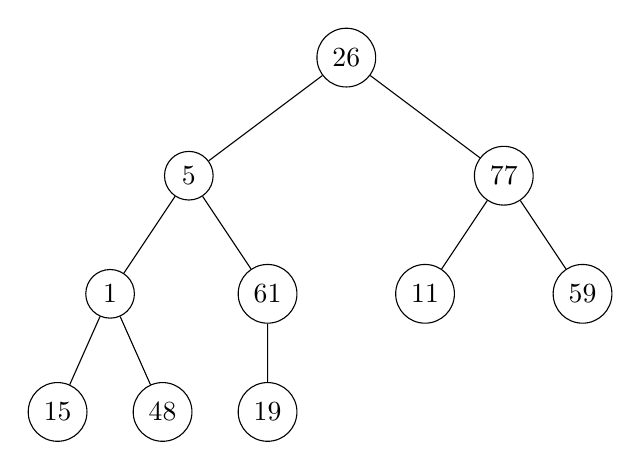
\begin{tikzpicture}[level/.style={sibling distance=40mm/#1}]
    \node[circle, draw] (z){$26$}
        child {node [circle, draw] (a) {$5$}
          child {node [circle, draw] (c) {$1$}
            child {node [circle, draw] (d) {$15$}}
            child {node [circle, draw] (f) {$48$}}
          }
          child {node [circle, draw] (e) {$61$}
            child {node [circle, draw] (f) {$19$}}
          }
        }
        child {node [circle, draw] (b) {$77$}
            child {node [circle, draw] (f) {$11$}}
            child {node [circle, draw] (f) {$59$}}
        }
;
\end{tikzpicture}
\column{0.3\textwidth}
\begin{tabular}{c | c |} \cline{2-2}
  [1]  & 26  \\ \cline{2-2}
  [2]  & 5   \\ \cline{2-2}
  [3]  & 77  \\ \cline{2-2}
  [4]  & 1   \\ \cline{2-2}
  [5]  & 61  \\ \cline{2-2}
  [6]  & 11  \\ \cline{2-2}
  [7]  & 59  \\ \cline{2-2}
  [8]  & 15  \\ \cline{2-2}
  [9]  & 48  \\ \cline{2-2}
  [10] & 19  \\ \cline{2-2}
\end{tabular}
\end{columns}

\end{frame}

\begin{frame}[t, fragile]
  \frametitle{Heap Sort}
Initial max heap construction
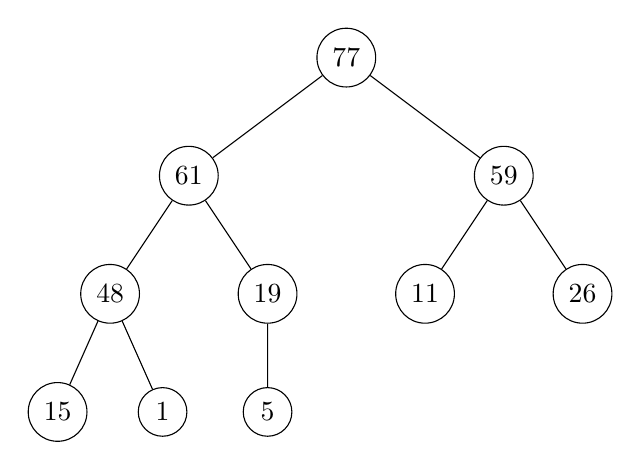
\begin{tikzpicture}[level/.style={sibling distance=40mm/#1}]
    \node[circle, draw] (z){$77$}
        child {node [circle, draw] (a) {$61$}
          child {node [circle, draw] (c) {$48$}
            child {node [circle, draw] (d) {$15$}}
            child {node [circle, draw] (f) {$1$}}
          }
          child {node [circle, draw] (e) {$19$}
            child {node [circle, draw] (f) {$5$}}
          }
        }
        child {node [circle, draw] (b) {$59$}
            child {node [circle, draw] (f) {$11$}}
            child {node [circle, draw] (f) {$26$}}
        }
;
\end{tikzpicture}


\end{frame}

\begin{frame}[t, fragile, allowframebreaks]
  \frametitle{Heap Sort: the code \texttt{(codes/heapsort.c)}}
    \lstinputlisting[firstnumber=28, firstline=28, lastline=64, basicstyle=\footnotesize]{codes/heapsort.c}
\end{frame}

%typo revivsed -44p KSS-
\begin{frame}[t]
  \frametitle{Heap Sort}
Time complexity:

$log_2n + log_2(n-1) + \cdots + log_22$
$=O(n\cdot log_2n)$
\end{frame}


\section{Radix Sort}
\begin{frame}[t]
  \frametitle{Radix Sort}
  \begin{itemize}
  \item It is a kind of distributive sort
  \item Repeats the following 3 steps
    \begin{enumerate}
    \item Comparison
    \item Distribution
    \item Merging
    \end{enumerate}

  \end{itemize}
\end{frame}


\begin{frame}[t]
  \frametitle{Radix Sort: Example}

Initial unsorted array

  \begin{center}
    \printarray[3em]{110, 12, 380, 2, 32, 41, 151, 253}
  \end{center}

First consider the One's place
  \begin{center}
$    \printarray[3em]{11\mathbf{0}, 1\mathbf{2}, 38\mathbf{0}, \mathbf{2}, 3\mathbf{2}, 4\mathbf{1}, 15\mathbf{1}, 25\mathbf{3}}$

$    \printarray[3em]{11\mathbf{0}, 38\mathbf{0}, 4\mathbf{1},  15\mathbf{1}, 1\mathbf{2}, \mathbf{2}, 3\mathbf{2},  25\mathbf{3}}$

  \end{center}

Consider the Ten's place
  \begin{center}
$    \printarray[3em]{1\mathbf{1}0, 3\mathbf{8}0, \mathbf{4}1, 1\mathbf{5}1, \mathbf{1}2,  2, \mathbf{3}2,   2\mathbf{5}3}$

$    \printarray[3em]{2, 1\mathbf{1}0, \mathbf{1}2, \mathbf{3}2,  \mathbf{4}1, 1\mathbf{5}1,      2\mathbf{5}3, 3\mathbf{8}0}$

  \end{center}

Consider the Hundred's place
  \begin{center}
$    \printarray[3em]{2, \mathbf{1}10, 12, 32,  41, \mathbf{1}51,      \mathbf{2}53, \mathbf{3}80}$

$    \printarray[3em]{2,  12, 32,  41, \mathbf{1}10, \mathbf{1}51,      \mathbf{2}53, \mathbf{3}80}$

  \end{center}


\end{frame}

\begin{frame}[t]
  \frametitle{Radix Sort: Time complexity}
Let there be $d$ digits in input integers.

In general, Radix sort takes $O(d\cdot (n+b))$ time where $b$ is the base of the given number.
\bigskip
Assume that $k = max(n)$, then $d = O(log_bk)$. The overall time complexity becomes $O((n+b)\cdot log_bk)$
\bigskip
If we further assume that $k = n^c$, where $c$ is constant, the time complexity becomes $O(n\cdot log_bn)$
\end{frame}


\end{document}
